 % =============================================================================
%  Presentation:
%  "The Role of AI Literacy in Trust Calibration toward AI-Generated Content"
%  Revised Questionnaire — Course Research Project
%
%  Compile with:  pdflatex ai_literacy_trust_presentation.tex   (twice)
% =============================================================================
\documentclass[10pt,aspectratio=169]{beamer}
\usepackage{comment}

% ------------------------------ Packages -------------------------------------
\usepackage[utf8]{inputenc}
\usepackage[T1]{fontenc}
\usepackage{lmodern}
\usepackage{tikz}
\usetikzlibrary{arrows.meta, positioning, shapes.geometric, fit, backgrounds}
\usepackage{booktabs}
\usepackage{array}
\usepackage{xcolor}

\usepackage{appendixnumberbeamer}

% ------------------------------ Custom colors --------------------------------
\definecolor{accent}{RGB}{35, 90, 130}
\definecolor{soft}{RGB}{230, 238, 247}

% ------------------------------ Theme ----------------------------------------
\usetheme[progressbar=frametitle, numbering=fraction, block=fill]{metropolis}
\setbeamertemplate{navigation symbols}{}
\setbeamercolor{progress bar}{fg=accent}
\setbeamercolor{frametitle}{bg=accent}
\setbeamercolor{title separator}{fg=accent}
\setbeamercolor{alerted text}{fg=accent}
\setbeamertemplate{page number in foot}[totalframenumber]

% ------------------------------ Custom commands ------------------------------
\newcommand{\presenter}[1]{}

% ------------------------------ Title page -----------------------------------
\title[AI Literacy \& Trust Calibration]%
{The Role of AI Literacy in Trust Calibration\\toward AI-Generated Content}
\subtitle{Course Research Project --- Questionnaire Presentation}
\author{Diogo Costa \and Madalena Martins \and Maja Skwaron \and Rafael Gufler}
\institute[]{Human-AI Interaction Course}
\date{May 13, 2026}

% =============================================================================
\begin{document}
% =============================================================================

% ---------------------------------------------------------------- Title ------
\begin{frame}[plain]
  \titlepage
\end{frame}

% ---------------------------------------------------------------- Outline ----
\begin{frame}{Outline}
  \small
  \begin{columns}[T]
    \column{0.5\textwidth}
    \textbf{Part 1 -- Research Design}
    \begin{itemize}
      \item Research question \& hypotheses
      \item Variables and constructs
    \end{itemize}
    \medskip
    \textbf{Part 2 -- Theoretical Background}
    \begin{itemize}
      \item AI literacy as a construct
      \item Trust in AI: HAITS
    \end{itemize}
    \column{0.5\textwidth}
    \textbf{Part 3 -- Instrument}
    \begin{itemize}
      \item Overview of the questionnaire
      \item Objective knowledge test (OLS)
      \item Trust subscales
    \end{itemize}
    \medskip
    \textbf{Part 4 -- Analysis \& Limitations}
    \begin{itemize}
      \item Analysis protocol
      \item Known limitations
    \end{itemize}
  \end{columns}
\end{frame}

% =============================================================================
\section{Part 1 -- Research Design}
% =============================================================================

% ---------------------------------------------------- 1. Research question ---
\begin{frame}{Research Question \& Hypotheses}
  \begin{block}{Research Question}
    Does \textbf{objective AI literacy} predict \textbf{trust in AI tools}
    among university students?
  \end{block}
  \pause
  \begin{alertblock}{Core argument}
    Users who understand how AI actually works --- probabilistic generation,
    hallucination tendencies, bias mechanisms, knowledge limits ---
    should be \textbf{less likely} to trust its outputs uncritically.
  \end{alertblock}
  \pause
  \begin{columns}[T]
    \column{0.5\textwidth}
    \begin{block}{H1 --- Competence Trust}
      Higher AI literacy $\Rightarrow$\\
      \textbf{lower} Competence Trust in AI tools.
    \end{block}
    \column{0.5\textwidth}
    \begin{block}{H2 --- Perceived Risk}
      Higher AI literacy $\Rightarrow$\\
      \textbf{higher} Perceived Risk when using AI tools.
    \end{block}
  \end{columns}
\end{frame}

% ---------------------------------------------------- 2. Variables -----------
\begin{frame}{Variables and Constructs}
  \centering
  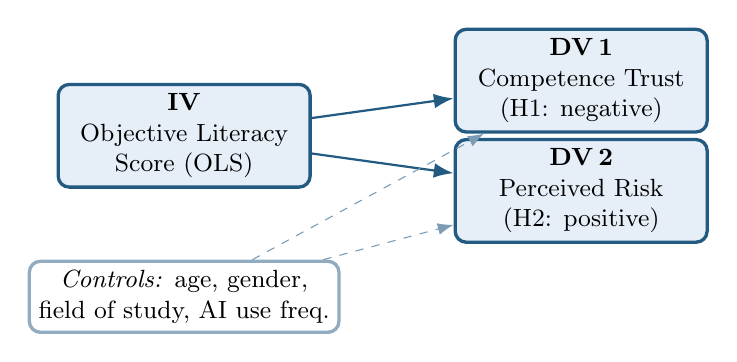
\begin{tikzpicture}[
      every node/.style={font=\small},
      box/.style={rectangle, draw=accent, very thick, fill=soft,
                  rounded corners, minimum height=1.1cm, minimum width=3.2cm,
                  align=center},
      arrow/.style={-{Latex[length=2.5mm]}, thick, draw=accent}
    ]
    \node[box] (iv) {\textbf{IV}\\ Objective Literacy\\ Score (OLS)};
    \node[box, right=1.8cm of iv, yshift=0.7cm] (dv1)
          {\textbf{DV\,1}\\ Competence Trust\\(H1: negative)};
    \node[box, right=1.8cm of iv, yshift=-0.7cm] (dv2)
          {\textbf{DV\,2}\\ Perceived Risk\\(H2: positive)};
    \node[box, below=0.9cm of iv, fill=white, draw=accent!50,
          minimum width=3.2cm, minimum height=0.9cm]
          (ctrl) {\small\textit{Controls:} age, gender,\\\small field of study, AI use freq.};

    \draw[arrow] (iv)   -- (dv1);
    \draw[arrow] (iv)   -- (dv2);
    \draw[-{Latex[length=2mm]}, dashed, draw=accent!60] (ctrl) -- (dv1);
    \draw[-{Latex[length=2mm]}, dashed, draw=accent!60] (ctrl) -- (dv2);
  \end{tikzpicture}
  \vspace{0.5em}
  \begin{exampleblock}{Exploratory (not hypothesis tests)}
    \textbf{Overconfidence gap}: self-estimated OLS minus actual OLS. Domain-specific trust: 8 contexts from low- to high-stakes.
    \quad
  \end{exampleblock}
\end{frame}

% =============================================================================
\section{Part 2 -- Theoretical Background}
% =============================================================================

% ---------------------------------------------------- 3. AI Literacy ---------
\begin{frame}{AI Literacy as a Construct}
  \begin{columns}[T]
    \column{0.55\textwidth}
    \begin{block}{Key definitions}
      \begin{itemize}
        \item \textbf{Long \& Magerko (2020, CHI):} AI literacy = competencies
              to critically evaluate, communicate with, and use AI.
        \item \textbf{Ng et al.\ (2022):} four domains --- knowing, using,
              evaluating, ethical AI.
        \item This study focuses on \textbf{objective} literacy:
              performance-based knowledge of how AI systems work.
      \end{itemize}
    \end{block}
    \column{0.45\textwidth}
    \begin{block}{Knowledge test source}
      \textbf{Hornberger et al.\ (2023)}\\
      \emph{Computers and Education: AI}
      \begin{itemize}
        \item Only peer-reviewed, IRT-validated AI literacy test.
        \item Validated on $N = 1{,}286$ German university students.
        \item This study: \textbf{11 items} translated to English.
      \end{itemize}
    \end{block}
  \end{columns}
\end{frame}

% ---------------------------------------------------- 4. Trust in AI ---------
\begin{frame}{Trust in AI: the HAITS}
  \begin{block}{Human-AI Trust Scale --- Sun et al.\ (2025)}
    Validated on $N = 1{,}426$ (China + US).
    Four factors: Affective Trust, \textbf{Competence Trust},
    Benevolence \& Integrity, \textbf{Perceived Risk}.
  \end{block}
  \pause
  \begin{columns}[T]
    \column{0.5\textwidth}
    \begin{block}{Competence Trust (used: H1)}
      Does the user believe AI is \textbf{accurate and reliable}?\\[4pt]
    \end{block}
    \column{0.5\textwidth}
    \begin{block}{Perceived Risk (used: H2)}
      Does the user believe AI \textbf{could cause harm or deception}?\\[4pt]
    \end{block}
  \end{columns}
  \medskip
  \begin{alertblock}{Why not all four subscales?}
    Affective Trust and Benevolence \& Integrity measure \emph{relational bonding}
    (e.g.\ ``AI is my close friend'') --- outside the scope of trust in AI-generated
    \emph{content}.
  \end{alertblock}
\end{frame}

% =============================================================================
\section{Part 3 -- Instrument}
% =============================================================================

% ---------------------------------------------------- 5. Questionnaire overview
\begin{frame}{Questionnaire Overview}
  \textbf{5 sections} $\approx$ 8--10 minutes. Target: university students.
  \medskip
  \begin{center}
  \begin{tabular}{clll}
    \toprule
    \textbf{Section} & \textbf{Content} & \textbf{Items} & \textbf{Role} \\
    \midrule
    1 & Demographics \& background & 6 & Controls \\
    2 & AI usage behaviour & 4 + 1 & Control + Exploratory \\
    3 & Objective AI knowledge test & 12 & \textbf{IV --- OLS + Exploratory} \\
    4 & Trust in AI tools (HAITS) & 11 + 1 & \textbf{DVs} \\
    5 & Domain-specific trust & 8 & Exploratory \\
    \bottomrule
  \end{tabular}
  \end{center}
  \pause
  \begin{exampleblock}{Two embedded attention checks}
    Item 2.4: ``What is 4 + 4? Please type the number.'' \quad
    Item 4.12: ``Please select `Agree' for this item.''\\
    Responses failing either check are excluded from analysis.
  \end{exampleblock}
\end{frame}

% ---------------------------------------------------- 6. OLS -----------------
\begin{frame}{Section 3 --- Objective Literacy Score (OLS)}
  \textbf{11 knowledge items} (Hornberger et al., 2023), grouped into four themes:
  \medskip
  \begin{columns}[T]
    \column{0.5\textwidth}
    \textbf{1. ML fundamentals}\\
    \small Quality of a model, supervised vs.\ unsupervised learning,
    training/test split.\\[6pt]
    \textbf{2. Human role in AI}\\
    \small How and to what extent humans influence ML outcomes.
    \column{0.5\textwidth}
    \textbf{3. How AI works}\\
    \small Goal-directedness, learning from large data, recommender
    systems.\\[6pt]
    \textbf{4. Limitations \& ethics}\\
    \small Unrepresentative training data, black-box problem,
    predictive policing risks.
  \end{columns}
  \vspace{0.6em}
  \begin{block}{Scoring}
    1 point per correct answer; 5 options per item including ``I don't know''.\\
    \textbf{OLS range: 0--11.} \quad
    Item 3.12: self-estimate (overconfidence gap = estimate $-$ OLS).
  \end{block}
\end{frame}

% ---------------------------------------------------- 7. Trust items ---------
\begin{frame}[shrink]{Section 4 --- HAITS Trust Items}
  \small
  \begin{columns}[T]
    \column{0.5\textwidth}
    \begin{block}{Competence Trust (4.1--4.6)}
      \textit{1 = Strongly disagree, 5 = Strongly agree}
      \begin{enumerate}
        \item The AI tools are reliable.
        \item AI tools are competent and perform their tasks well.
        \item AI tools perform their role very well.
        \item AI tools can do everything I would expect them to.
        \item I can trust the information presented to me by AI tools.
        \item AI tools are fast and efficient.
      \end{enumerate}
    \end{block}
    \column{0.5\textwidth}
    \begin{block}{Perceived Risk (4.7--4.11) --- all reverse-coded (R)}
      \textit{1 = Strongly disagree, 5 = Strongly agree}
      \begin{enumerate}
        \setcounter{enumi}{6}
        \item The AI tools are deceptive. (R)
        \item The AI tools behave in an underhanded manner. (R)
        \item I am suspicious of the AI tools' intent or outputs. (R)
        \item The AI tools' actions could lead to harmful outcomes. (R)
        \item It is risky to interact with AI tools. (R)
      \end{enumerate}
    \end{block}
  \end{columns}
  \vspace{0.4em}
  \begin{exampleblock}{Scoring note}
    For Perceived Risk, higher scores indicate that students see AI tools as more risky, which reflects lower trust.
  \end{exampleblock}
\end{frame}

% ---------------------------------------------------- 8. Domain trust --------
\begin{frame}{Section 5 --- Domain-Specific Trust}
  \textbf{8 domains} rated on: \textit{1 = Not at all, 5 = Completely}\\[4pt]
  Informed by Nguyen et al.\ (2025) --- AI trust and literacy in student samples.
  \vspace{0.5em}

  \begin{columns}[T]
    \column{0.48\textwidth}
    \begin{block}{Lower-stakes domains}
      \begin{itemize}
        \item General knowledge questions
        \item Learning or study-related tasks
        \item Programming or technical tasks
        \item Professional or work-related tasks
      \end{itemize}
    \end{block}
    \column{0.48\textwidth}
    \begin{alertblock}{Higher-stakes domains}
      \begin{itemize}
        \item Writing academic work (essays, papers)
        \item \textbf{Health-related questions}
        \item \textbf{Personal advice or life decisions}
        \item News and current events
      \end{itemize}
    \end{alertblock}
  \end{columns}
  \vspace{0.5em}
  \begin{exampleblock}{Exploratory purpose}
    If H1 and H2 hold, literacy effects are expected to be strongest in high-stakes domains - where the cost of misplaced trust is highest - and weakest in low-stakes domains.
  \end{exampleblock}
\end{frame}

% =============================================================================
\section{Part 4 -- Analysis \& Limitations}
% =============================================================================
 
% ---------------------------------------------------- 9a. Analysis Steps 1-2 ---
\begin{frame}{Analysis Protocol --- Steps 1 \& 2}
  \begin{columns}[T]
    \column{0.5\textwidth}
    \begin{block}{Step 1 --- Data preparation}
      \begin{itemize}
        \item \textbf{Exclude} responses failing either attention check.
        \item \textbf{Exclude} bottom 5th percentile completion times\\
              {\footnotesize (implausibly fast = not reading carefully)}
        \item \textbf{Score OLS} (0--11): 1 = correct, 0 = incorrect or ``I don't know''.
        \item \textbf{Reverse-code} Perceived Risk items 4.7--4.11\\
              {\footnotesize (subtract from 6, so high score = high risk)}
        \item \textbf{Overconfidence gap} = item 3.12 $-$ actual OLS\\
              {\footnotesize (positive = overconfident; reported descriptively)}
      \end{itemize}
    \end{block}
    
    \column{0.5\textwidth}
    \begin{block}{Step 2 --- Scale reliability}
      \begin{itemize}
        \item Compute \textbf{Cronbach's $\alpha$} and \textbf{McDonald's $\omega$}
              for both subscales.\\
              {\footnotesize $\alpha/\omega$ measure whether items in a scale
              consistently point at the same construct. Target: $\alpha \geq .70$.}
        \item \textbf{Benchmarks from Sun et al.\ (2025):}\\
              Competence Trust $\omega = .966$\\
              Perceived Risk $\omega = .959$
        \item If $\alpha < .70$: inspect item-total correlations; remove weakest item.
        \item If $N \geq 150$: optional \textbf{two-factor CFA} in \texttt{lavaan}\\
              {\footnotesize confirms the two-factor structure holds in our sample;
              report CFI, RMSEA, SRMR}
      \end{itemize}
    \end{block}
  \end{columns}
\end{frame}
 
% ---------------------------------------------------- 9b. Analysis Steps 3-4 ---
\begin{frame}{Analysis Protocol --- Steps 3 \& 4}

\begin{columns}[T,onlytextwidth]

  \begin{column}{0.48\textwidth}
    \begin{block}{Step 3 --- Descriptives}
    \scriptsize
      \begin{itemize}
        \item Means and SDs for all constructs.

        \item \textbf{Correlation matrix}: check that OLS correlates negatively
        with Competence Trust and positively with Perceived Risk before
        running regressions.

        \item \textbf{One-sample $t$-test} on overconfidence gap vs.\ zero:
        
        tests whether students systematically over- or underestimate their own
        AI knowledge.
      \end{itemize}
    \end{block}
  \end{column}

  \begin{column}{0.48\textwidth}
    \begin{block}{Step 4 --- Hypothesis testing}
    \scriptsize

      Two \textbf{multiple regressions}, one per hypothesis.

      \medskip

      \textbf{H1:} OLS $\rightarrow$ Competence Trust
      
      Expected: $\beta < 0$

      \medskip

      \textbf{H2:} OLS $\rightarrow$ Perceived Risk
      
      Expected: $\beta > 0$

      \medskip

      Both models control for age, gender, field of study, and AI use frequency.

      \medskip

      Controls remove variance explained by, for example, STEM students having
      both higher literacy and different trust baselines.

      \medskip

      \textbf{Report:} standardized $\beta$, $R^2$, $p$-value, Cohen's $f^2$.

      \medskip

      $f^2 = .02$ small; $.15$ medium; $.35$ large.

    \end{block}
  \end{column}

\end{columns}

\vspace{0.3em}

\begin{exampleblock}{Target sample size}
\scriptsize
Minimum $N \approx 85$ with power $= .80$, $f^2 = .15$, and 4 predictors.

Aim for $N = 100$--$150$.

Pre-register on OSF before data collection.
\end{exampleblock}

\end{frame}

% ---------------------------------------------------- 9c. Sample size --------
\begin{frame}[t]{Sample Size}
\footnotesize

\begin{block}{Power analysis}
\vspace{-0.3em}
\begin{itemize}
  \setlength\itemsep{0.2em}

  \item Two multiple regressions with 4 predictors.

  \item Assumed effect size: $f^2 = .15$ (medium), based on the
  AI literacy--attitude literature.

  \item At power $= .80$ and $\alpha = .05$: 
  \textbf{minimum $N \approx 85$}.

  \item \textbf{Target: $N = 100$--$150$} to allow for exclusions
  such as attention-check failures or very fast completions.

\end{itemize}
\vspace{-0.4em}
\end{block}

\vspace{-0.25em}

\end{frame}

% ---------------------------------------------------- 10. Limitations --------
\begin{frame}{Known Limitations (Pre-Acknowledged)}
  \small
  \begin{enumerate}
    \item \textbf{No dispositional trust control.}
          Baseline technology enthusiasm is not measured; field of study and
          prior AI coursework serve as proxy controls. Future work should
          include a validated dispositional trust scale (McKnight et al., 2011).

    \item \textbf{Cross-linguistic transfer of knowledge items.}
          Hornberger et al.'s test was developed in German; IRT item parameters
          may not transfer directly to an English-language sample. Item-level
          descriptives will characterize the scale empirically.

    \item \textbf{Partial HAITS.}
          Only two of four subscales used (Competence Trust + Perceived Risk).
          Affective Trust and Benevolence \& Integrity are out of scope but
          relevant for future research on heavy AI users.

    \item \textbf{Student sample.}
          University students have above-average digital literacy; variance in
          both literacy and trust may be compressed relative to the general
          population.
  \end{enumerate}
\end{frame}

% =============================================================================
\section{Appendix A -- Construct Map}
% =============================================================================

% ---------------------------------------------------- App A: construct map ---
\begin{frame}{Appendix A --- Construct Map (Controls \& Exploratory)}
  \small
  \begin{tabular}{lllp{3.6cm}}
    \toprule
    \textbf{Items} & \textbf{Construct} & \textbf{Role} & \textbf{Source} \\
    \midrule
    1.1--1.2 & Age, gender            & Control            & Brown et al.\ (2025) \\
    1.3--1.4 & Field of study, status & Control            & Hornberger et al.\ (2023) \\
    1.5      & AI course experience   & Control            & KPMG (2025) \\
    1.6      & AI usage duration      & Control            & Developed for study \\
    \midrule
    2.1      & AI use frequency       & Control            & Brown et al.\ (2025) \\
    2.2      & Weekly AI time         & Control            & Developed for study \\
    2.3 + 2.5    & Self-rated confidence  & \textit{Exploratory} --- overconfidence gap & DSIT (2026); KPMG (2025) \\
    \midrule
    3.1--3.11 & Objective AI literacy & \textbf{Main IV --- H1 \& H2} & Hornberger et al.\ (2023) \\
    3.12     & Self-estimated score   & \textit{Exploratory} --- overconfidence gap & Welsch et al.\ (2025) \\
    \midrule
    4.1--4.6  & Competence Trust      & \textbf{Primary DV --- H1} & Sun et al.\ (2025) HAITS \\
    4.7--4.11 & Perceived Risk (R)    & \textbf{Primary DV --- H2} & Sun et al.\ (2025) HAITS \\
    \midrule
    5.1--5.8  & Domain-specific trust & \textit{Exploratory} & Nguyen et al.\ (2025) \\
    \bottomrule
  \end{tabular}
\end{frame}

% =============================================================================
\begin{comment}
\section{Appendix B -- Analysis Protocol}
\end{comment}
% =============================================================================

% ---------------------------------------------------- App B: full steps ------
\begin{comment}
\begin{frame}{Appendix B --- Full Analysis Protocol}
  \small
  \begin{columns}[T]
    \column{0.5\textwidth}
    \textbf{Step 1 --- Data preparation}\\
    Exclude attention-check failures \& bottom 5th-percentile completion times.
    Reverse-score items 4.7--4.11. Score OLS (0--11).
    Compute overconfidence gap = item 3.12 $-$ OLS.
    \medskip

    \textbf{Step 2 --- Reliability \& dimensionality}\\
    $\alpha$ and $\omega$ for both subscales; compare to Sun et al.\ benchmarks.
    Aggregate if $\alpha \geq .70$; else inspect item-total correlations.
    Optional two-factor CFA in \texttt{lavaan} if $N \geq 150$ (report CFI, RMSEA, SRMR).
    Compute Trust Differentiation Index = SD of items 5.1--5.8 per respondent.
    \medskip

    \textbf{Step 3 --- Descriptives}\\
    Means, SDs, bivariate correlation matrix, normality tests.
    One-sample $t$-test (or Wilcoxon) on overconfidence gap vs.\ zero.

    \column{0.5\textwidth}
    \textbf{Step 4 --- Hypothesis tests}
    \begin{itemize}
      \item \textbf{H1:} OLS $\rightarrow$ Competence Trust mean (expected $\beta < 0$).
      \item \textbf{H2:} OLS $\rightarrow$ Perceived Risk mean (expected $\beta > 0$).
      \item Both regressions: controls = age, gender, field of study, AI use frequency.
      \item Report standardized $\beta$, $R^2$, $p$, Cohen's $f^2$.
    \end{itemize}
    \medskip

    \textbf{Step 5 --- Domain analysis (descriptive)}\\
    Report mean trust per domain (5.1--5.8).
    Paired $t$-tests: high-stakes (5.6, 5.7) vs.\ low-stakes (5.1, 5.4).
    Bonferroni-correct if comparing $>2$ domains.
    \medskip

    \textbf{Step 6 --- Reporting}\\
    Min.\ $N \approx 85$ (power = .80, $f^2 = .15$); target $N = 100$--$150$.
    Pre-register on OSF before data collection.
    Report item-level OLS difficulty (proportion correct); flag floor/ceiling effects ($>85\%$).
  \end{columns}
\end{frame}
\end{comment}

% =============================================================================
\section{Appendix B -- Key References}
% =============================================================================

% ---------------------------------------------------- App C: references ------
\begin{frame}{Appendix B --- Key References}
  \scriptsize
  \begin{itemize}
    \item Brown, R., Sillence, E., \& Branley-Bell, D. (2025). AcademAI: Investigating AI usage,
          attitudes, and literacy in higher education and research.
          \textit{Journal of Educational Technology Systems}, 54(1), 6--33.

    \item Department for Science, Innovation and Technology \& DCMS. (2026).
          \textit{AI skills for life and work: General public survey findings}. GOV.UK.

    \item Hornberger, M., Bewersdorff, A., \& Nerdel, C. (2023). What do university students know
          about Artificial Intelligence? Development and validation of an AI literacy test.
          \textit{Computers and Education: Artificial Intelligence}, 5, 100165.

    \item Koch, M.\ J., et al.\ (2024). Meta AI literacy scale: Further validation and development
          of a short version. \textit{Heliyon}, 10(21), e39686.

    \item KPMG International \& University of Melbourne. (2025).
          \textit{Trust, attitudes and use of artificial intelligence: A global study 2025}.

    \item Long, D., \& Magerko, B. (2020). What is AI literacy? Competencies and design
          considerations. \textit{Proceedings of CHI 2020}, 1--16.

    \item Mayer, R.\ C., Davis, J.\ H., \& Schoorman, F.\ D. (1995). An integrative model of
          organizational trust. \textit{Academy of Management Review}, 20(3), 709--734.

    \item Ng, D.\ T.\ K., et al.\ (2022). Conceptualizing AI literacy: An exploratory review.
          \textit{Computers and Education: Artificial Intelligence}, 2, 100041.

    \item Nguyen, N.\ B., et al.\ (2025). Learning with algorithms: AI usage, trust, and literacy
          among university students. \textit{HCMC Open University Journal of Science}, 16(10).

    \item Sun, H., et al.\ (2025). Revisiting trust in the era of generative AI: Factorial structure
          and latent profiles. arXiv:2510.10199.

    \item Welsch, R., et al.\ (2025). AI makes you smarter but none the wiser.
          \textit{Computers in Human Behavior}, 168, 108262.
  \end{itemize}
\end{frame}

% ---------------------------------------------------- 12. Q\&A ---------------
\begin{frame}[plain]
  \vfill
  \centering
  {\Huge\bfseries Thank you!}\\[1em]
  {\Large Questions?}\\[2em]
  \footnotesize
  \textit{The Role of AI Literacy in Trust Calibration toward AI-Generated Content}\\
  Course Research Project --- Questionnaire Presentation
  \vfill
\end{frame}

\end{document}
